
\chapter{Datasets}
\label{ch:data}


\section{Dataset 1}
\label{sec:data1}

The Dataset 1 \cite{wiki} contains 100 persons \ldots 
In Fig.~\ref{fig:data1} four examples are illustrated:
In Fig.~\ref{fig:data1}\subref{subfig:data1_p1} person 1 smiles \ldots 

\begin{figure}[htb]
    \centering
    %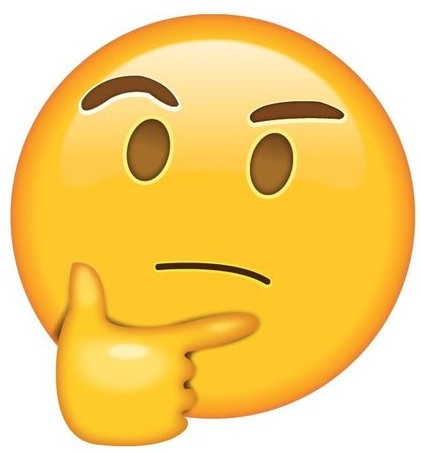
\includegraphics[width=0.3\textwidth]{figs/dummy_img}
    \subfloat[person 1 ]{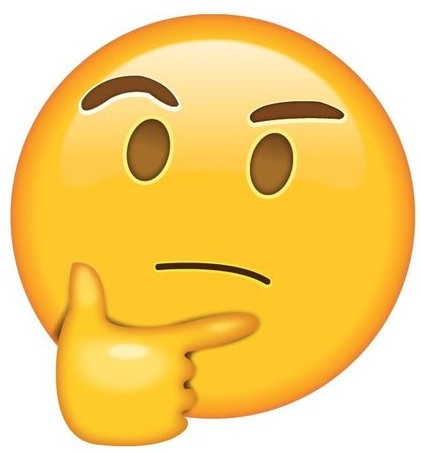
\includegraphics[width=0.24\textwidth]{figs/dummy_img}\label{subfig:data1_p1}}
    \subfloat[person 2 ]{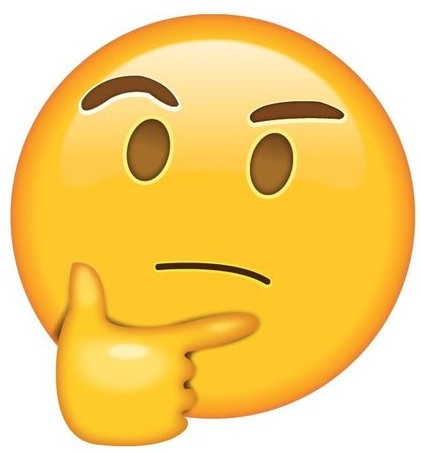
\includegraphics[width=0.24\textwidth]{figs/dummy_img}\label{subfig:data1_p2}}
    \subfloat[person 3 ]{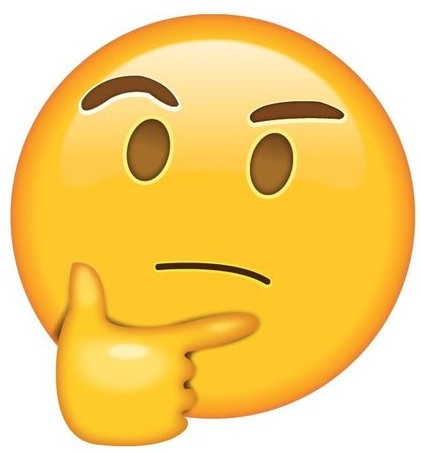
\includegraphics[width=0.24\textwidth]{figs/dummy_img}\label{subfig:data1_p3}}\\
    \subfloat[person 4 ]{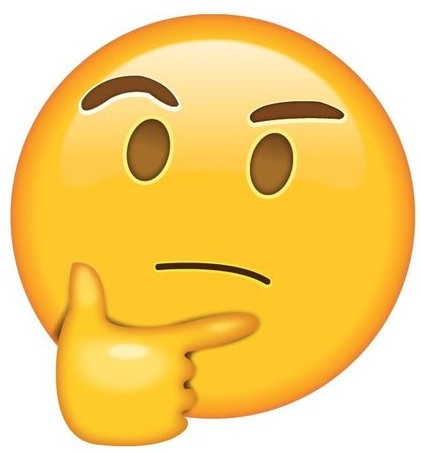
\includegraphics[width=0.24\textwidth]{figs/dummy_img}\label{subfig:data1_p4}}\\

    \caption{Samples from Dataname, with varying persons: \protect\subref{subfig:data1_p1}: smile, \protect\subref{subfig:data1_p2} person 2 frowns,  \protect\subref{subfig:data1_p3} shows Tom Hanks, \protect\subref{subfig:data1_p4} fancy stuff.}
    \label{fig:dataset1}
\end{figure}


